\documentclass[a4j,10pt]{jsarticle}
\usepackage{layout,url,resume}
\usepackage[dvipdfmx]{graphicx}
\pagestyle{empty}

\begin{document}
%\layout

\title{Emscriptenを用いたx86エミュレータのブラウザへの移植}

% 和文著者名
\author{
	Arch B1 坂本優太(sksat)
}

% 和文概要
\begin{abstract}
Emscriptenというフレームワークを用い,
以前自作したx86エミュレータをブラウザへの移植を行った.
\end{abstract}

\maketitle
\thispagestyle{empty}

\section{背景}
近年,WebAssemblyという,ブラウザ上で動作するアセンブリ風の低水準言語の開発が進められている.
これにより,ブラウザ上でネイティブアプリケーション並の高速な計算を行うことができる.

WebAssemblyはLLVM 8.0\footnote{2019/03/20リリース}で正式なターゲットとしてサポートされたこともあり,
今後様々な場面で使われていくだろうと思われる.

また,EmscriptenというLLVMを用いたフレームワークを用いることで,
比較的簡単にC/C++で記述されたプログラムをブラウザ向けにビルドすることが可能になっている.

そこで,あらゆるプラットフォームでの動作を目的として,
今回は以前C++で開発したx86エミュレータをEmscriptenによりブラウザへ移植することを考えた.

\section{関連研究}
WebAssemblyを用いてエミュレータをブラウザ上で動作させるという発想は以前からあるもので,
関連研究として,JSLinux\footnote{https://bellard.org/jslinux/}
やv86\footnote{http://copy.sh/v86/}などが挙げられる.

JSLinuxはQEMUの開発者であるFabrice Bellardが開発したもので,
x86/riscv64をターゲットにしたLinux KernelやWindows 2000などをブラウザ上でエミュレーションすることができる.

v86はターゲットアーキテクチャはx86のみだが,
複数のLinux DistributionやWindows 1.0などのエミュレーションが可能であり,
起動時にディスクイメージを指定することもできる.

\section{移植したエミュレータ}
今回移植したエミュレータは高校2年生の頃にフルスクラッチで開発したもので,
ソースコードはGitHubで公開している\footnote{https://github.com/sk2sat/emu}.

このエミュレータのターゲットアーキテクチャはx86であり,
ユーザーアプリケーションの動作ではなく,
「はりぼてOS」という教育用の小さなOSを動作させることを開発目標としていた.
そのため,このエミュレータではまずフロッピーイメージを読み込み,
16bitリアルモード,一部のBIOSファンクション,32bitプロテクトモード
のエミュレーションをすることができる\footnote{ただし,ページングはサポートしておらず,セグメンテーションについてもメモリ保護機能はほとんど実装されていない.}.

\begin{figure}[htbp]
	\begin{center}
		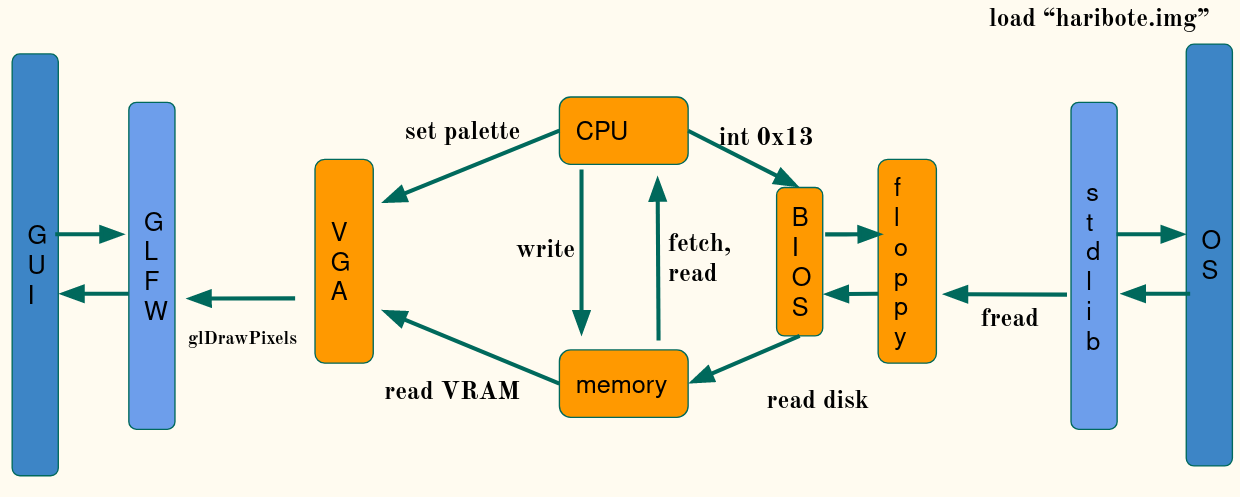
\includegraphics[width=7.5cm]{./emu_struct.png}
		\caption{自作エミュレータの構造}
		\label{emustruct}
	\end{center}
\end{figure}

\section{実装}
EmscriptenはWebAssembly向けのコンパイラだけではなく,
標準ライブラリやOpenGLなどの一部のライブラリをJavaScriptに移植したものを含んでいる.
そのため,それらのライブラリのみを使用したアプリケーションはC/C++のコンパイラを"emcc"に指定するだけでブラウザ向けにビルドすることができる.

しかし,それだけでは自作のエミュレータを移植することはできなかった.
これにより移植できたのは図\ref{emustruct}の中央のオレンジ色で示した部分にとどまった.

\subsection{ファイル読み込み}
\subsection{GUI}
% pthreadがexperimental
% glDrawPixelsが使えない
% emscripten_loopが使えない
% 最終的にやったこと

\section{考察}

\bibliographystyle{junsrt}
\bibliography{resume}

\end{document}
% end of file
